%!TEX root = ../template.tex
%%%%%%%%%%%%%%%%%%%%%%%%%%%%%%%%%%%%%%%%%%%%%%%%%%%%%%%%%%%%%%%%%%%%
%% chapter4.tex
%% NOVA thesis document file
%%
%% Chapter with lots of dummy text
%%%%%%%%%%%%%%%%%%%%%%%%%%%%%%%%%%%%%%%%%%%%%%%%%%%%%%%%%%%%%%%%%%%%
\chapter{Simulación}
\label{cha:Simulación}

\section{Infraestructura} % (fold)
\label{sec:Infraestructura}


Con el fin de definir el comportamiento del diseño planteado se realizaron simulaciones de los dos escenarios, tanto de sedes remotas como de sedes nacionales, para asegurar que la red se comporta tal como se predijo y que se están cumpliendo los requisitos de la disponibilidad y calidad de servicio.

\subsection{Infraestructura Utilizada para la Simulación} % (fold)
\label{sec:Infraestructura Utilizada para la Simulación}

La simulación se realizó utilizando el software GNS3, sin embargo dados los requerimientos de protocolos y dado que se requería de equipos que soporten IWAN no se utilizó GNS3 en su modo tradicional emulando routers directamente en su plataforma, por el contrario se creó una máquina virtual Ubuntu cuyo objetivo es realizar la virtualización de equipos de red, por lo que la simulación fue realizada con VNF creando una máquina virtual para cada uno de los routers simulados, se utiliza por tanto el concepto de virtualización anidada de forma que cada router virtual se crea como una máquina virtual dentro de otra máquina virtual, el esquema de esta virtualización \textbf{Ver figura 12.1 Infraestructura Utilizada para la Simulación}.
\begin{figure}[htbp]
  \centering
  %\subcaptionbox{\label{fig:leftsubfig}}%
    {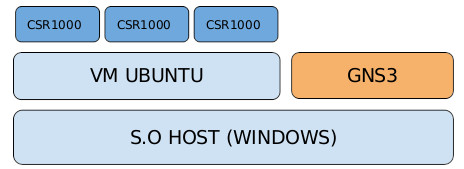
\includegraphics[width=0.7\linewidth]{figure44}}%
%  \subcaptionbox{Another sub-figure\label{fig:rightsubfig}}%
%    {
\includegraphics[width=0.5\linewidth]{knitting-vectorial}}%
  \caption{Infraestructura Utilizada para la Simulación}
  \label{fig:fig2subfig}
\end{figure}
Esta virtualización Anidada se realizó utilizando VMware workstation pro, mediante esta herramienta se virtualizó la VM de Ubuntu dentro del sistema operativo Windows, a su vez dentro de esta máquina virtual de Ubuntu se utilizó virtualización KVM para montar cada uno de los enrutadores virtuales.
\\
\\
Esta configuración permite por un lado mantener contenidos dentro de la máquina virtual Ubuntu los recursos que utilizan los enrutadores virtuales de manera que la utilización de estas máquinas no colapse el sistema operativo host al dejar sin recursos el sistema operativo y permite por otro lado integrar GNS3 con routers VNF reales, en este caso los CSR1000v de Cisco que están diseñados específicamente para servicios en la nube y soportan todas las características requeridas por la solución de IWAN. Estos enrutadores virtuales requieren 1 core y 3GB de RAM, por tanto la simulación se realizó en un equipo con las siguientes carácteristicas técnicas:

\begin{table}[ht]
	\caption{Amazon EC2 Pricing.}
	\label{tab:hla:results}
\centering
\begin{tabular}{lccccc}
	\toprule
	\multicolumn{1}{c}{\textbf{Proceso}} 	& \textbf{IWAN}	& \textbf{Tiempo}	& \textbf{Solución Actual}
	& \textbf{Tiempo}\\
	\midrule
\cite{Aprovisionamiento tienda nueva} 		& N/A & 2GiB & EBS Only	& \$0.0255 per Hour \\
\cite{a1.large}~2 		& N/A & 4GiB & EBS Only & \$0.051 per Hour	\\
\cite{a1.xlarge}~4		& N/A & 4GiB & EBS Only & \$0.051 per Hour	\\
\cite{a1.2xlarge}~8 	& N/A & 16GiB & EBS Only & \$0.204 per Hour	\\
\cite{a1.4xlarge}~16	& N/A & 32GiB & EBS Only & \$0.408 per Hour	\\
\cite{t3.nano}~2		& N/A & 0.5GiB & EBS Only & \$0.0052 per Hour	\\
\cite{t3.micro}~2   	& N/A & 1GiB & EBS Only & \$0.0104 per Hour	\\
	\midrule
	\textbf{Total}			& \textbf{--}		& \textbf{--}		& \textbf{--} \\
	\bottomrule
\end{tabular}
\end{table}

De estos recursos tuvieron que asignarse 12MB de memoria RAM para la máquina virtual ya que cada uno de los routers requiere 3MB de Memoria para funcionar correctamente y 4 threads de procesamiento de los 8 disponibles para el procesamiento requerido por los enrutadores, por otra lado solamente 8GB de disco duro fueron suficientes para esta máquina virtual.

\subsection{Topologías y Configuraciones Realizadas} % (fold)
\label{sec:Topologías y Configuraciones Realizadas}

Dado el diseño planteado se realizaron pruebas con dos topologías diferentes, la primera siendo la topología de las sedes nacionales, es decir dos CPE en la sede cada uno recibiendo un hilo de fibra por un transporte diferente. Para esta topología se incluyeron un total de 5 enrutadores, dos realizando la función de HBR (Hub Border Router) que actúan como Hubs para los túneles en la topología DMVPN y un MC(Master Controller) encargado de establecer las políticas de PfR de cada una de las aplicaciones y propagar las políticas por el resto de la red.\textbf{Ver figura 12.2 La topología configurada en GNS3}.
\begin{figure}[htbp]
  \centering
  %\subcaptionbox{\label{fig:leftsubfig}}%
    {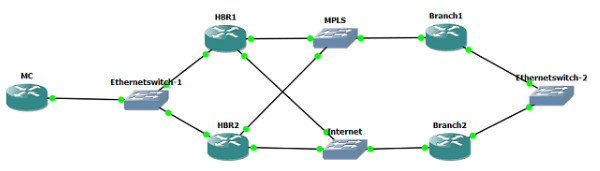
\includegraphics[width=0.9\linewidth]{figure45}}%
%  \subcaptionbox{Another sub-figure\label{fig:rightsubfig}}%
%    {
\includegraphics[width=0.5\linewidth]{knitting-vectorial}}%
  \caption{La topología configurada en GNS3 }
  \label{fig:fig2subfig}
\end{figure}

En la topología se simulan los diferentes transportes con switches, uno para la MPLS y otro para el transporte de internet, esto es una simplificación de las redes de transporte reales ya que estas son mucho más complejas, pero en este caso la simulación mantiene su validez ya que para establecer los túneles que funcionan acá como la red “underlay” únicamente se requiere conectividad IP entre los routers Branch y los HBR sin importar la forma como esta se de.

Como se mencionó anteriormente los HBR actúan como Hubs para la topología DMVPN y en esta topología los dos equipos Branch se registran contra dichos equipos como lo muestra \textbf{Ver figura 12.3 Branch1} para el Branch1 y \textbf{Ver figura 12.4 Branch2} para el Branch2

\begin{figure}[htbp]
  \centering
  %\subcaptionbox{\label{fig:leftsubfig}}%
    {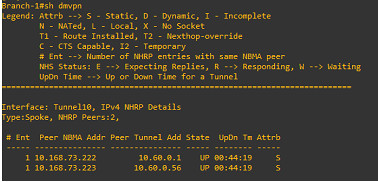
\includegraphics[width=0.7\linewidth]{figure46}}%
%  \subcaptionbox{Another sub-figure\label{fig:rightsubfig}}%
%    {
\includegraphics[width=0.5\linewidth]{knitting-vectorial}}%
  \caption{Branch1}
  \label{fig:fig2subfig}
\end{figure}


\begin{figure}[htbp]
  \centering
  %\subcaptionbox{\label{fig:leftsubfig}}%
    {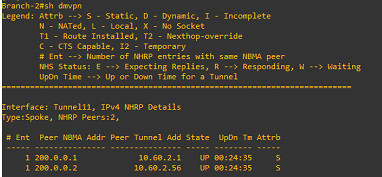
\includegraphics[width=0.7\linewidth]{figure47}}%
%  \subcaptionbox{Another sub-figure\label{fig:rightsubfig}}%
%    {
\includegraphics[width=0.5\linewidth]{knitting-vectorial}}%
  \caption{Branch2}
  \label{fig:fig2subfig}
\end{figure}

Además de estas adyacencias de DMVPN se configuró EIGRP como protocolo de enrutamiento utilizado tanto hacia los túneles como entre los routers Branch y en datacenter entre los HBR y el MC, las \textbf{Ver figura 12.5 Configuración EIGRP} y \textbf{Ver figura 12.6 Configuración EIGRP} muestran los establecimientos de dichas adyacencias en el Branch.

\begin{figure}[htbp]
  \centering
  %\subcaptionbox{\label{fig:leftsubfig}}%
    {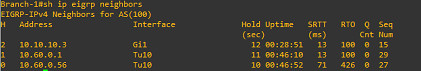
\includegraphics[width=0.7\linewidth]{figure48}}%
%  \subcaptionbox{Another sub-figure\label{fig:rightsubfig}}%
%    {
\includegraphics[width=0.5\linewidth]{knitting-vectorial}}%
  \caption{Configuración EIGRP}
  \label{fig:fig2subfig}
\end{figure}


\begin{figure}[htbp]
  \centering
  %\subcaptionbox{\label{fig:leftsubfig}}%
    {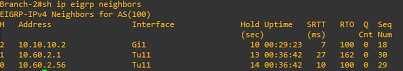
\includegraphics[width=0.7\linewidth]{figure49}}%
%  \subcaptionbox{Another sub-figure\label{fig:rightsubfig}}%
%    {
\includegraphics[width=0.5\linewidth]{knitting-vectorial}}%
  \caption{Configuración EIGRP}
  \label{fig:fig2subfig}
\end{figure}

Finalmente el otro componente que hace parte de la solución de IWAN es PfR, en este caso uno de los routers (El activo en la configuración de HSRP) toma el rol de master en PFR encargándose de distribuir las políticas a los border router del Branch, las imagenes \textbf{Ver figura 12.7 Registros de los Routers}y \textbf{Ver figura 12.8 Registros de los Routers} muestran el registro de los dos routers con PfR.

\begin{figure}[htbp]
  \centering
  %\subcaptionbox{\label{fig:leftsubfig}}%
    {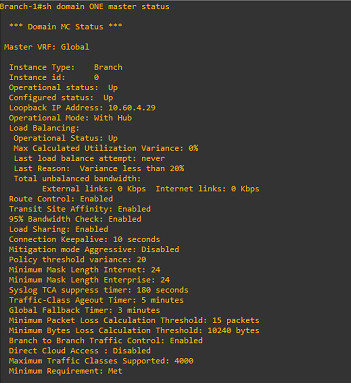
\includegraphics[width=0.5\linewidth]{figure50}}%
%  \subcaptionbox{Another sub-figure\label{fig:rightsubfig}}%
%    {
\includegraphics[width=0.5\linewidth]{knitting-vectorial}}%
  \caption{Registros de los Routers}
  \label{fig:fig2subfig}
\end{figure}


\begin{figure}[htbp]
  \centering
  %\subcaptionbox{\label{fig:leftsubfig}}%
    {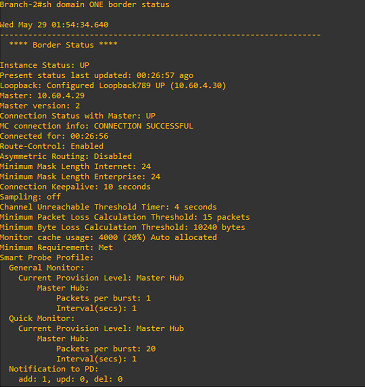
\includegraphics[width=0.5\linewidth]{figure51}}%
%  \subcaptionbox{Another sub-figure\label{fig:rightsubfig}}%
%    {
\includegraphics[width=0.5\linewidth]{knitting-vectorial}}%
  \caption{Registros de los Routers}
  \label{fig:fig2subfig}
\end{figure}

El diseño para las sedes regionales difiere de las sedes nacionales en cuanto a que por costos no se utilizan dos routers sino uno sólo con dos métodos de transporte independientes, en este sentido la distribución y configuración de la topología en datacenter se mantiene exactamente igual, el único cambio de configuración se realiza sobre el router Branch, la topología simulada para este caso es ilustrada en la figura \textbf{Ver figura 12.9 Topología Router Branch}

\begin{figure}[htbp]
  \centering
  %\subcaptionbox{\label{fig:leftsubfig}}%
    {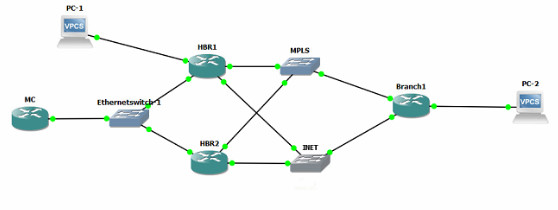
\includegraphics[width=0.9\linewidth]{figure52}}%
%  \subcaptionbox{Another sub-figure\label{fig:rightsubfig}}%
%    {
\includegraphics[width=0.5\linewidth]{knitting-vectorial}}%
  \caption{Topología Router Branch}
  \label{fig:fig2subfig}
\end{figure}

En este caso el único router branch contará con 4 adyacencias de DMVPN, dos por cada HBR, correspondientes a los diferentes tipos de transporte. Esto asegura que hay redundancia en caso de que alguno de los HBR falle o en caso de ruptura de fibra óptica para alguno de los canales de transporte. la imagen \textbf{Ver figura 12.10 Registro desde el Router} ilustra la forma como se ve este registro desde el router.

\begin{figure}[htbp]
  \centering
  %\subcaptionbox{\label{fig:leftsubfig}}%
    {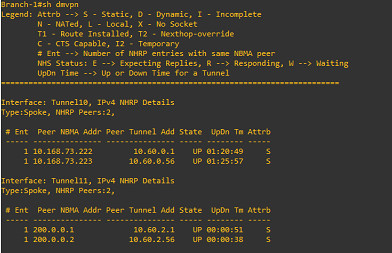
\includegraphics[width=0.6\linewidth]{figure53}}%
%  \subcaptionbox{Another sub-figure\label{fig:rightsubfig}}%
%    {
\includegraphics[width=0.5\linewidth]{knitting-vectorial}}%
  \caption{  Registro desde el Router}
  \label{fig:fig2subfig}
\end{figure}

De igual forma a pesar de que se forman adyacencias EIGRP por los túneles GRE multipunto únicamente contra los 2 HBR se establecen 4 vecindades de HSRP diferentes, dos por cada HBR, este comportamiento puede verse más claramente en el router como lo muestra la figura \textbf{Ver figura 12.11 Adyacencias EIGRP por los Túneles GRE}

\begin{figure}[htbp]
  \centering
  %\subcaptionbox{\label{fig:leftsubfig}}%
    {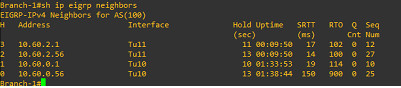
\includegraphics[width=0.5\linewidth]{figure54}}%
%  \subcaptionbox{Another sub-figure\label{fig:rightsubfig}}%
%    {
\includegraphics[width=0.5\linewidth]{knitting-vectorial}}%
  \caption{  Adyacencias EIGRP por los Túneles GRE}
  \label{fig:fig2subfig}
\end{figure}

En cuanto al protocolo PfR el mismo router cumple las funciones de master y de borde para el branch, registrándose y descargando las políticas desde el MC en el datacenter. La imagen \textbf{Ver figura 12.12  Protocolo PfR} muestra dicho registro.

\begin{figure}[htbp]
  \centering
  %\subcaptionbox{\label{fig:leftsubfig}}%
    {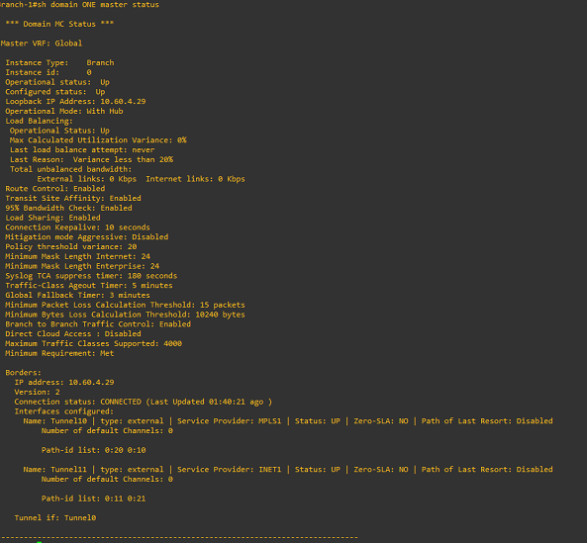
\includegraphics[width=0.5\linewidth]{figure55}}%
%  \subcaptionbox{Another sub-figure\label{fig:rightsubfig}}%
%    {
\includegraphics[width=0.5\linewidth]{knitting-vectorial}}%
  \caption{  Protocolo PfR}
  \label{fig:fig2subfig}
\end{figure}
